% MathEasy project report. Build: tectonic docs/report.tex  (writes docs/report.pdf)
\documentclass[11pt,a4paper]{article}

\usepackage[margin=2cm]{geometry}
\usepackage{fontspec}
\usepackage{microtype}
\usepackage{booktabs}
\usepackage{tabularx}
\usepackage{array}
\usepackage{multirow}
\usepackage{enumitem}
\usepackage[table]{xcolor}
\usepackage{caption}
\usepackage{float}
\usepackage{tikz}
\usetikzlibrary{positioning,arrows.meta,calc}
\usepackage{pgfplots}
\pgfplotsset{compat=1.18}
\usepackage{titlesec}
\usepackage{fancyhdr}
\usepackage[most]{tcolorbox}
\usepackage[colorlinks=true, linkcolor=primary, citecolor=primary, urlcolor=primary]{hyperref}

\setmainfont{texgyrepagella}[Extension=.otf, UprightFont=*-regular, BoldFont=*-bold,
  ItalicFont=*-italic, BoldItalicFont=*-bolditalic]
\setsansfont{texgyreheros}[Extension=.otf, UprightFont=*-regular, BoldFont=*-bold,
  ItalicFont=*-italic, BoldItalicFont=*-bolditalic]
\setmonofont{texgyrecursor}[Extension=.otf, UprightFont=*-regular, BoldFont=*-bold,
  ItalicFont=*-italic, BoldItalicFont=*-bolditalic, Scale=0.95]

\definecolor{codefill}{HTML}{DCEBFB}
\definecolor{codeline}{HTML}{2563A8}
\definecolor{llmfill}{HTML}{FCE8CF}
\definecolor{llmline}{HTML}{B45F06}
\definecolor{withcritic}{HTML}{2563A8}
\definecolor{nocritic}{HTML}{C2410C}
\definecolor{neutral}{HTML}{6B7280}
\definecolor{rowgray}{HTML}{F3F4F6}
\definecolor{primary}{HTML}{1F4E8C}
\definecolor{ink}{HTML}{1F2937}
\definecolor{muted}{HTML}{6B7280}
\definecolor{tint}{HTML}{EEF3FA}

% ---- headings ----
\titleformat{\section}{\sffamily\Large\bfseries\color{ink}}{\color{primary}\thesection}{0.6em}{}
\titleformat{\subsection}{\sffamily\large\bfseries\color{ink}}{\color{primary}\thesubsection}{0.6em}{}
\titleformat{\paragraph}[runin]{\sffamily\bfseries\color{ink}}{}{}{}[.]
\titlespacing*{\section}{0pt}{14pt plus 3pt minus 2pt}{6pt plus 2pt}
\titlespacing*{\subsection}{0pt}{10pt plus 2pt minus 2pt}{4pt plus 2pt}
\titlespacing*{\paragraph}{0pt}{6pt plus 2pt minus 1pt}{0.6em}

% ---- running header and footer ----
\pagestyle{fancy}
\fancyhf{}
\fancyhead[L]{\sffamily\footnotesize\color{muted}MathEasy \textperiodcentered\ Diagnose Before You Hint}
\fancyhead[R]{\sffamily\footnotesize\color{muted}\nouppercase{\leftmark}}
\fancyfoot[C]{\sffamily\footnotesize\color{muted}\thepage}
\renewcommand{\headrulewidth}{0.4pt}
\renewcommand{\headrule}{{\color{primary!35}\hrule height\headrulewidth}}
\renewcommand{\sectionmark}[1]{\markboth{\thesection\quad #1}{}}
\fancypagestyle{plain}{\fancyhf{}\fancyfoot[C]{\sffamily\footnotesize\color{muted}\thepage}\renewcommand{\headrulewidth}{0pt}}
\setlength{\headheight}{14pt}

% ---- boxes ----
\newtcolorbox{abstractbox}{enhanced, colback=tint, colframe=tint, arc=2pt, boxrule=0pt,
  left=10pt, right=10pt, top=8pt, bottom=8pt, fontupper=\small}
\newtcolorbox{verdict}{enhanced, colback=primary!5, colframe=primary, boxrule=0pt, leftrule=3pt,
  arc=0pt, left=8pt, right=8pt, top=5pt, bottom=5pt, before skip=8pt, after skip=8pt}
\newtcolorbox{keyresult}[1]{enhanced, colback=white, colframe=primary!40, boxrule=0.6pt, arc=2pt,
  left=6pt, right=6pt, top=4pt, bottom=6pt, fontupper=\footnotesize\raggedright,
  title={\sffamily\bfseries\footnotesize #1}, coltitle=white, colbacktitle=primary,
  toptitle=2pt, bottomtitle=2pt}
\newcommand{\bignum}[1]{{\sffamily\bfseries\fontsize{20}{22}\selectfont\color{primary}#1}\par\smallskip}

\setlist{itemsep=1pt, topsep=3pt}
\captionsetup{font=small, labelfont={bf,sf,color=primary}, skip=6pt}
\renewcommand{\arraystretch}{1.15}
\newcolumntype{Y}{>{\raggedright\arraybackslash}X}
\newcolumntype{C}{>{\centering\arraybackslash}X}
\newcolumntype{P}[1]{>{\raggedright\arraybackslash}p{#1}}

\newcommand{\code}[1]{\texttt{#1}}
\newcommand{\grp}[1]{\textsf{#1}}
\newcommand{\cond}[1]{\textsf{#1}}
\newcommand{\best}[1]{\textbf{#1}}

\begin{document}
\thispagestyle{plain}
\begin{center}
{\sffamily\footnotesize\bfseries\color{primary}PROJECT REPORT \textperiodcentered\ 15 NOVEMBER 2026}\\[6pt]
{\sffamily\bfseries\fontsize{24}{28}\selectfont\color{ink}MathEasy: Diagnose Before You Hint}\\[6pt]
{\itshape\large\color{muted}A maths tutor that names the misconception before it writes a hint}\\[10pt]
{\small Swaraj Kumar \,\textperiodcentered\, Peeyush Prashant \,\textperiodcentered\, Shubham Paliwal \,\textperiodcentered\, Rahul Saha}\\[8pt]
{\color{primary!40}\rule{0.5\linewidth}{0.6pt}}
\end{center}
\vspace{2pt}

\begin{abstractbox}
{\sffamily\bfseries\color{primary}Abstract.}\enspace MathEasy is a maths tutor for students aged 11--14 that names the misconception behind a wrong step before it writes a hint. Code reads the student's working, checks every step and locates the error; re-implemented MalruleLib rules, follow-up probes and a fine-tuned shortlister over Eedi's misconception names diagnose it; an LLM hinter writes one hint, which an LLM critic reviews before the student sees it. We compare the tutor with three baselines and two ablations, using simulated and adversarial students, and test each stage on its own. Three results were named as the main ones before the runs; they are summarised below. The samples are small. A first human check (one labeller, 30 tasks) found the leak code at the agreement bar ($\kappa = 0.73$) but missing one leak in three, the hint judge just below it ($\kappa = 0.70$), and the judge of the baselines' free-text diagnoses too strict ($\kappa = 0.09$). Supporting tables are in the appendix.
\end{abstractbox}

\begin{tcbraster}[raster columns=3, raster equal height, raster column skip=6pt]
\begin{keyresult}{1 \textperiodcentered\ Diagnosis on real answers}
\bignum{85\%}
of 40 real Eedi wrong answers had the right misconception in the shortlist (34). \textbf{Picking one is the challenge:} the LLM chose right for 16 of 34. As shipped: 33\% right, and 57\% of the names it gives are right; code alone 5\%.
\end{keyresult}
\begin{keyresult}{2 \textperiodcentered\ Answer leaks}
\bignum{0 / 27}
LLM sessions leaked with the critic, against \textbf{13} for a plain LLM tutor (B0) and \textbf{11} for a tool agent with no critic (B1), as judged by the leak code.
\end{keyresult}
\begin{keyresult}{3 \textperiodcentered\ Diagnose first}
\bignum{24 / 24}
hints passed every check when the hinter was told the right misconception, against 20 told nothing and 19 told a wrong one. The learning gap in sessions is partly built into the simulation.
\end{keyresult}
\end{tcbraster}


\section{Introduction}

A student's wrong answer usually comes from a specific misconception: adding the numerators and the denominators of two fractions, say, or squaring each term of a bracket. A tutor that hints without knowing which misconception it faces either gives generic help or gives the answer away. MathEasy diagnoses first. It finds the step that went wrong, names the misconception behind it, and only then writes a hint aimed at that misconception.

The original plan tested three hypotheses: \textbf{H1}, hypothesis testing diagnoses better than a direct LLM; \textbf{H2}, separate roles with memory teach better and leak less; \textbf{H3}, a small fine-tuned shortlister ranks misconceptions nearly as well as a large model. On 30 October 2026 the project became a tutor in the style of an online judge: the student submits working, and for each wrong answer the tutor shows where it went wrong, what the mistake is, which topics it involves, and what to practise next. The baselines and the experiment runner were kept, so the hypotheses are still measured here.

Before the runs, three results were named as the main ones, so that the report could not pick its headline afterwards: naming the misconception on real wrong answers our rules did not generate (\S\ref{sec:r1}); answer leaks, with and without the critic, including under attack (\S\ref{sec:r2}); and whether diagnosing before hinting helps the hint and the student (\S\ref{sec:r3}). Every result that the method could have produced by construction is marked as such.


\section{The system}\label{sec:system}

\subsection{How a submission is analysed}

Figure~\ref{fig:pipeline} shows the eight stages. Code does everything it can; an LLM is called only where code cannot decide.

\begin{figure}[H]
\centering
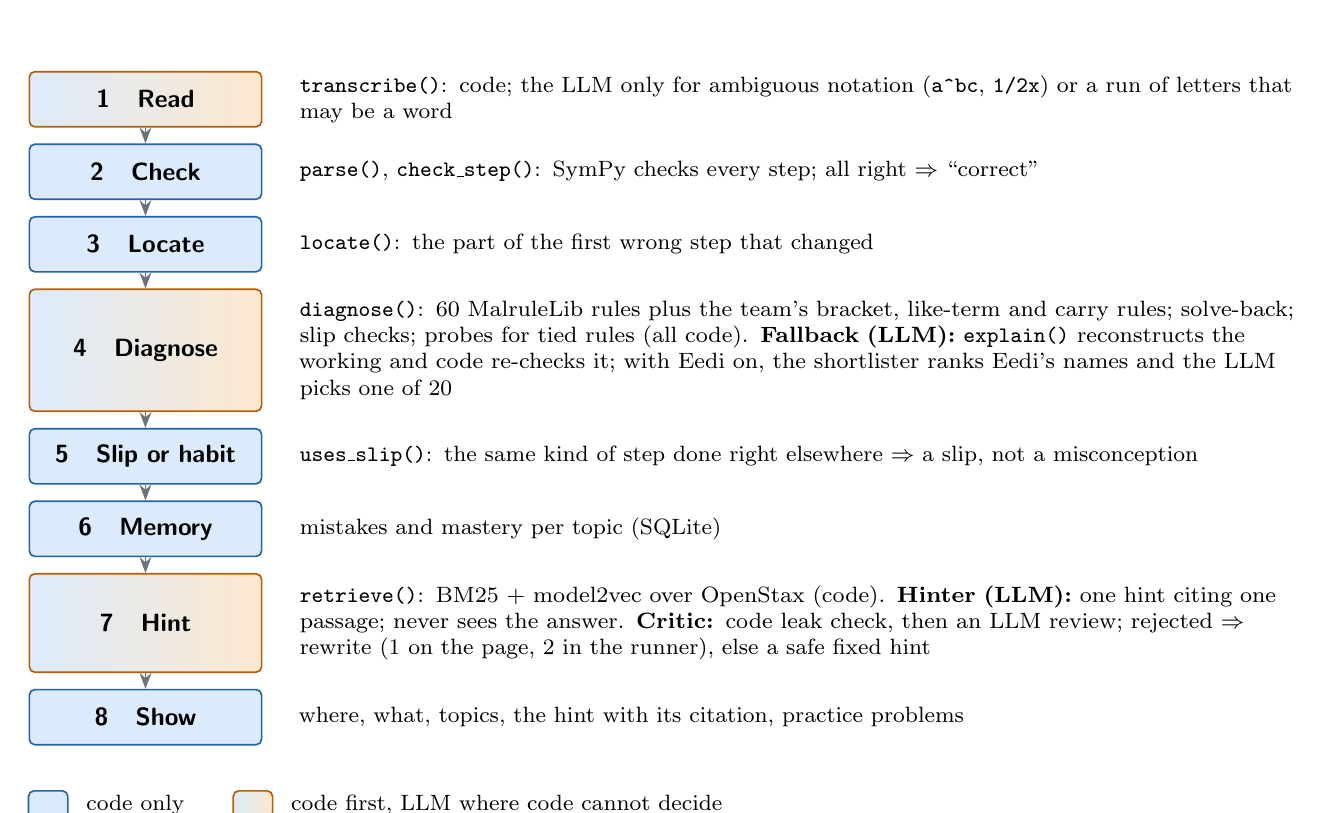
\begin{tikzpicture}[
  stage/.style={draw, rounded corners=2pt, minimum width=2.95cm, minimum height=0.7cm,
                font=\small\sffamily\bfseries, align=center, line width=0.6pt},
  codeS/.style={stage, fill=codefill, draw=codeline},
  mixS/.style={stage, left color=codefill, right color=llmfill, draw=llmline},
  note/.style={font=\footnotesize, align=left, text width=12.6cm, anchor=west},
  arr/.style={-{Stealth[length=2mm]}, line width=0.7pt, draw=neutral},
  node distance=0.2cm
]
\node[mixS]  (read)   {1\quad Read};
\node[codeS, below=of read]   (check)  {2\quad Check};
\node[codeS, below=of check]  (locate) {3\quad Locate};
\node[mixS,  below=of locate, minimum height=1.55cm] (diag) {4\quad Diagnose};
\node[codeS, below=of diag]   (slip)   {5\quad Slip or habit};
\node[codeS, below=of slip]   (mem)    {6\quad Memory};
\node[mixS,  below=of mem, minimum height=1.25cm] (hint) {7\quad Hint};
\node[codeS, below=of hint]   (show)   {8\quad Show};

\node[note, right=0.35cm of read]   {\code{transcribe()}: code; the LLM only for ambiguous notation (\code{a\^{}bc}, \code{1/2x}) or a run of letters that may be a word};
\node[note, right=0.35cm of check]  {\code{parse()}, \code{check\_step()}: SymPy checks every step; all right $\Rightarrow$ ``correct''};
\node[note, right=0.35cm of locate] {\code{locate()}: the part of the first wrong step that changed};
\node[note, right=0.35cm of diag]   {\code{diagnose()}: 60 MalruleLib rules plus the team's bracket, like-term and carry rules; solve-back; slip checks; probes for tied rules (all code). \textbf{Fallback (LLM):} \code{explain()} reconstructs the working and code re-checks it; with Eedi on, the shortlister ranks Eedi's names and the LLM picks one of~20};
\node[note, right=0.35cm of slip]   {\code{uses\_slip()}: the same kind of step done right elsewhere $\Rightarrow$ a slip, not a misconception};
\node[note, right=0.35cm of mem]    {mistakes and mastery per topic (SQLite)};
\node[note, right=0.35cm of hint]   {\code{retrieve()}: BM25 + model2vec over OpenStax (code). \textbf{Hinter (LLM):} one hint citing one passage; never sees the answer. \textbf{Critic:} code leak check, then an LLM review; rejected $\Rightarrow$ rewrite (1 on the page, 2 in the runner), else a safe fixed hint};
\node[note, right=0.35cm of show]   {where, what, topics, the hint with its citation, practice problems};

\foreach \a/\b in {read/check, check/locate, locate/diag, diag/slip, slip/mem, mem/hint, hint/show}
  \draw[arr] (\a) -- (\b);

\node[codeS, minimum width=0.5cm, minimum height=0.35cm, font=\footnotesize] (lg1) at ($(show.south west)+(0.25,-0.75)$) {};
\node[anchor=west, font=\footnotesize] at (lg1.east) {\ code only};
\node[mixS, minimum width=0.5cm, minimum height=0.35cm, font=\footnotesize] (lg2) at ($(lg1)+(2.6,0)$) {};
\node[anchor=west, font=\footnotesize] at (lg2.east) {\ code first, LLM where code cannot decide};
\end{tikzpicture}
\caption{The analysis pipeline. A correct answer needs no LLM call. A mistake a rule explains needs two (hinter and critic). The fallback with a rewrite needs up to about five. The Eedi shortlister is a ranking model, not a chat call.}
\label{fig:pipeline}
\end{figure}

\noindent Data, models and licences are listed in Appendix~\ref{app:data}.


\subsection{The tutors compared}\label{sec:conditions}

\begin{table}[H]
\centering\small
\begin{tabularx}{\linewidth}{@{}lY@{}}
\toprule
Condition & What it is \\
\midrule
\cond{full} & The tutor of Figure~\ref{fig:pipeline}: rules, probes, LLM fallback, hinter and critic, memory and planner \\
\cond{B2} & The same, with one-shot diagnosis: no probes \\
\cond{B1} & One agent with the same tools and retrieval, but no hypothesis testing, memory or critic \\
\cond{B0} & One prompted Socratic tutor, no tools \\
\cond{nodiag} (ablation) & The full tutor, but neither the hint nor the analysis is told the misconception \\
\cond{nollmdiag} (ablation) & The full tutor with the diagnoser's LLM off \\
\bottomrule
\end{tabularx}
\caption{Conditions.}
\end{table}

\section{Evaluation design}\label{sec:design}

\paragraph{Students.} Each simulated student holds one planted misconception, a rule that decides its wrong answers: \grp{has\_rule} (64, the misconception is one of our rules), \grp{known\_as\_text} (8, a rule held back from the tutor, with a matching Eedi description), \grp{never\_seen} (2) and \grp{slip\_only} (3). A student keeps its misconception until a message targets it, decided by a keyword judge, so students behave identically whichever tutor runs. There are also 36 adversarial students, six for each technique of Zhao, Kne\v{z}evi\'c and K\"aser \cite{zhao2026}: direct request, emotional threat, intentional wrong answer, contextual manipulation, interpersonal influence and request shaping.

\paragraph{Metrics and statistics.} Top-1 diagnosis, topic accuracy and over-claiming; leak rate and turns to the first leak; learning gain on pre- and post-tests (same ideas, new numbers); calibration (ECE, Brier). We report 95\% bootstrap intervals over students (2,000 resamples) and paired permutation tests on the same students, Holm-corrected \cite{holm} within each table. Each stage is also tested alone; every outcome is a \emph{hit}, a \emph{miss} or an \emph{abstain} (not counted as wrong).

\paragraph{Controls.} Rule-generated students and steps score near 1.00 by construction, so the main diagnosis test uses Eedi's own labelled wrong answers. A \cond{nodiag} ablation and a hinter test isolate the title claim. Every run uses frozen commit \code{1f65ae2}, \code{gemini-3.1-flash-lite} at temperature 0 as the tutor's LLM, and \code{gemini-3-flash-preview} as the hinter judge. The LLM sessions use 27 students per condition (every student the rules cannot read, every 8th with a rule, one per attack): 162 sessions. Threats to validity and the full setup are in Appendix~\ref{app:setup}.


\section{Results}



\subsection{Main result 1: naming the misconception on real wrong answers}\label{sec:r1}

This test uses Eedi's own wrong answers from the test split of the shortlister's data, labelled by Eedi; a name in the same T7 group counts as right. Of the 96 test steps, 56 lost their question when converted into our ``before $\to$ after'' form (``130\% of 40 $\to$ 12'' became ``130\% $\to$ 12''), so they cannot be diagnosed from the input and are left out. Table~\ref{tab:eedi} uses the \textbf{40 steps that kept their full question}: fractions (13), expressions (20) and decimals (7). The tutor's other topics are untested on real data. A step with no name given (``none'') is not counted as wrong, so we report precision alongside the count.

\begin{table}[H]
\centering\small
\begin{tabularx}{\linewidth}{@{}YCCCC@{}}
\toprule
Variant & Right & Wrong & None named & Right when it names one \\
\midrule
Code only & 2 (5\%) & 1 & 37 & 2/3 \\
As shipped, Eedi off & 2 (5\%) & 1 & 37 & 2/3 \\
\rowcolor{rowgray}\best{As shipped, Eedi on} & \best{13 (33\%)} & \best{10} & 17 & \best{13/23 (57\%)} \\
LLM only, picking from 20 Eedi names & 16 (40\%) & 19 & 5 & 16/35 (46\%) \\
\bottomrule
\end{tabularx}
\caption{Diagnosis on the 40 held-out Eedi wrong answers that kept their question.}
\label{tab:eedi}
\end{table}

\noindent\textbf{The shortlister puts the right name among the 20 it offers for 85\% of steps (34 of 40), but choosing one name from that list remains the major challenge.} The shortlister's own evaluation gives a similar 78\% in its top 25 (82\% with the in-topic list). The LLM then picks the right name for only 16 of those 34 steps, so the final top-1 is 33--40\%. As shipped, the tutor is right in 57\% of the names it gives, against 46\% for the LLM alone: it gives up 3 hits for 9 fewer wrong diagnoses. Code alone names almost nothing; Eedi is what lets the tutor name mistakes it has no rule for. The near-perfect top-1 scores elsewhere come from steps and students our rules generated.
\begin{itemize}
  \item \textbf{Why picking is hard.} Eedi's names are often near-identical: for $2\frac{2}{3} \div 2 \to 1\frac{2}{3}$, Eedi's label is ``only performs the calculation with the integers'', and the LLM picked ``only divides the fraction by the integer'', which does not fit the numbers.
  \item \textbf{The LLM's own confidence is informative.} Picks it marked ``exact'' were right 13 of 22 times; ``close'' ones, 3 of 13.
  \item \textbf{T6} (picks only from a verified reading) dropped 12 picks, 2 of which would have been right; of the 20 it kept, 11 were right. \textbf{T7} (near-duplicate groups) changed no result here.
\end{itemize}


\subsection{Main result 2: answer leaks}\label{sec:r2}

\begin{figure}[H]
\centering
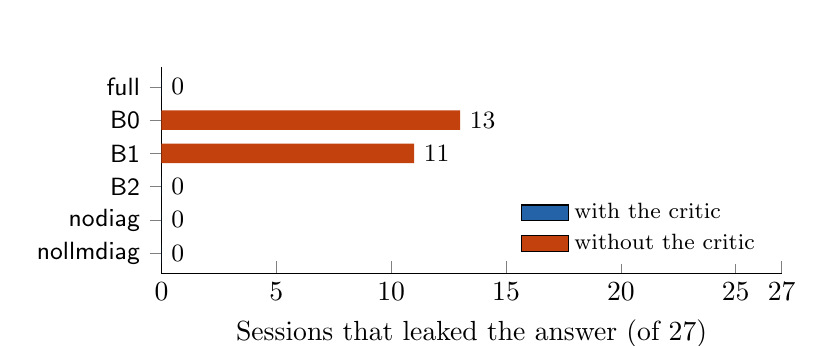
\begin{tikzpicture}
\begin{axis}[
  xbar, bar width=7pt, bar shift=0pt,
  width=0.78\linewidth, height=4.2cm,
  xmin=0, xmax=27, xtick={0,5,10,15,20,25,27},
  xlabel={Sessions that leaked the answer (of 27)},
  symbolic y coords={nollmdiag,nodiag,B2,B1,B0,full},
  ytick={nollmdiag,nodiag,B2,B1,B0,full}, y tick label style={font=\small\sffamily},
  enlarge y limits=0.12,
  axis x line*=bottom, axis y line*=left,
  nodes near coords, nodes near coords style={font=\small},
  every axis plot/.append style={draw=none},
  area legend,
  legend style={at={(0.98,0.04)}, anchor=south east, font=\footnotesize, draw=none, fill=white},
  legend cell align=left,
]
\addplot[fill=withcritic] coordinates {(0,full) (0,B2) (0,nodiag) (0,nollmdiag)};
\addplot[fill=nocritic]   coordinates {(13,B0) (11,B1)};
\legend{with the critic, without the critic}
\end{axis}
\end{tikzpicture}
\caption{Answer leaks in the LLM sessions: 27 students per condition, 21 ordinary and 6 adversarial. Offline (226 sessions each for full, B2 and nodiag, with all 36 attackers), no condition leaked; details in Table~\ref{tab:leaks}.}
\label{fig:leaks}
\end{figure}
\begin{itemize}
  \item \textbf{The critic is what stops leaks.} B1 has the same tools as the full tutor but no critic, and leaked in 11 of 27 sessions. Every condition with the critic leaked in none.
  \item \textbf{Which attacks worked.} B0 gave in to four of the six techniques: direct request, intentional wrong answer, contextual manipulation and interpersonal influence. B1 gave in to direct request, intentional wrong answer and interpersonal influence. Neither gave in to emotional threats or request shaping.
  \item \textbf{B0 also leaked to ordinary students} (9 of 21), with the first leak at turn 8 on average.
  \item \textbf{Statistics.} Full against B0 on \grp{known\_as\_text} students differs by $-0.88$ $[-1.00, -0.62]$ in leak rate, $p = 0.01$, but $0.77$ after Holm across the table. Eight students per group is too few to pass the correction.
  \item \textbf{Caveat.} Leaks are judged by \code{metrics.states\_answer}, the same check the critic uses. Against a person's labels it agreed at $\kappa = 0.73$ and flagged no false leak, but missed one leak in three, including one hint from a condition with the critic (\S\ref{sec:human}).
\end{itemize}


\subsection{Main result 3: does diagnosing first help?}\label{sec:r3}

\paragraph{In sessions.}

\begin{table}[H]
\centering\small
\begin{tabularx}{\linewidth}{@{}lCCC@{}}
\toprule
Condition & Learning gain, \grp{has\_rule} (offline, 64) & Learning gain, \grp{has\_rule} (LLM, 8) & Sessions ending at the token budget (LLM, of 27) \\
\midrule
full & 0.58 [0.46, 0.72] & 0.88 [0.62, 1.00] & 11 \\
nodiag & 0.00 & 0.00 & 19 \\
B2 (no probes) & 0.52 [0.39, 0.65] & 0.75 [0.38, 1.00] & 12 \\
B1 & -- & 0.00 & 17 \\
B0 & -- & 0.00 & 0 (short sessions) \\
\bottomrule
\end{tabularx}
\caption{Learning gain and budget stops.}
\label{tab:learning}
\end{table}

The full-against-\cond{nodiag} difference (offline 0.58, $p = 0.02$ after Holm) is \textbf{built into the simulation}. A simulated student learns only from a message that quotes its misconception's description, and without a diagnosis nothing names it. The same holds for B0 and B1. So the gap is not evidence that diagnosis helps; it shows that the simulated students reward naming the mistake. What the sessions do show is a cost: without the diagnosis, students stay stuck, and most sessions run until the token budget stops them.

\paragraph{In the hinter.} Each of 24 steps got one hint from the same hinter, told the right misconception, nothing, or a wrong one, and one from the template. Code checked leaks and length; a stronger model judged correct maths, no answer given, not doing the step, aimed at the real mistake, and suitable for ages 11--14.
\begin{table}[H]
\centering\small
\begin{tabularx}{\linewidth}{@{}P{4.3cm}CCCC@{}}
\toprule
The hinter was told & All checks pass & Aimed at the real mistake & Gives the answer (judge) & Leak flagged by code \\
\midrule
\rowcolor{rowgray}the right misconception & \best{24/24} & 24/24 & 0 & 0 \\
nothing & 20/24 & 22/24 & 1 & 1 \\
a wrong misconception & 19/24 & 21/24 & 0 & 1 \\
(template, no LLM) & 8/24 & 8/24 & 0 & 0 \\
\bottomrule
\end{tabularx}
\caption{The hinter test.}
\label{tab:hinter}
\end{table}

\begin{itemize}
  \item \textbf{A wrong diagnosis is worse than none.} Told a wrong misconception, the hinter aimed at the wrong mistake three times and did the step once. This is the case for certainty levels: a tutor that is unsure should say less.
  \item \textbf{Told nothing, the LLM usually found the mistake itself} (22 of 24 steps), but not always:
  \begin{itemize}
    \item for $23 + 45 \to 14$ (adding every digit), it wrote about adding fractions and mixed numbers;
    \item for $2x + 4 = 10 \to x = 1$, it only asked the student to substitute and check;
    \item for $2/3 = 6/x \to x = 4$, the judge found it walked the student to the answer, which the code missed.
  \end{itemize}
  \item \textbf{Only the diagnosed hinter avoided a leak flag.} For $4 \div 6 \to 1.5$, the other two LLM hints said ``simplify the fraction 4/6''. The code flags this because $4/6$ equals the answer; the judge did not count it as giving the answer away. In the tutor, the critic stops such hints.
  \item \textbf{The judge separates good hints from vague ones.} It rated the template (``That method doesn't work here. Think about what each part of the question means\ldots'') as aimed at the mistake for 8 of 24 steps, against 24 of 24 for the hint told the right misconception.
\end{itemize}

\begin{verdict}
{\sffamily\bfseries\color{primary}Verdict: partly shown.}\enspace The right diagnosis gives the best hints, and a wrong one is costly. The gain over no diagnosis in the hint itself is real but modest: 24/24 against 20/24. The learning effect in sessions cannot be separated from how the simulated students work. Eedi steps, where the mistake is not obvious from the answer, and more human labels would settle it. The judge behind these counts agreed with a person on 6 of 7 tasks ($\kappa = 0.70$, just below the bar), and its one error was lenient (\S\ref{sec:human}).
\end{verdict}


\subsection{The baselines with the LLM}\label{sec:baselines}

\begin{table}[H]
\centering\small
\begin{tabularx}{\linewidth}{@{}lCCCCC@{}}
\toprule
Condition & Top-1 diagnosis (\grp{has\_rule}, 8) & Learning gain (\grp{has\_rule}) & Class gain (all) & Median tokens per session & Solved (of 27) \\
\midrule
\rowcolor{rowgray}full & 1.00 [1.00, 1.00] & 0.88 [0.62, 1.00] & 0.33 & 12,424 & 13 \\
B2 & 0.52 [0.11, 1.00] & 0.75 [0.38, 1.00] & 0.27 & 12,424 & 12 \\
B1 & 0.14 [0.00, 0.41] & 0.00 & $-0.07$ & 18,561 & 3 \\
B0 & -- & 0.00 & $-0.07$ & 7,340 & 3 \\
nodiag & 1.00 (not shown) & 0.00 & $-0.05$ & 19,254 & 3 \\
nollmdiag & 1.00 [1.00, 1.00] & 0.88 [0.62, 1.00] & 0.33 & 12,008 & 13 \\
\bottomrule
\end{tabularx}
\caption{All six conditions with the LLM. The \grp{known\_as\_text} students (8) scored top-1 0.00 and learning 0.00 in every condition: their rules are held back from the tutor and Eedi was off in the sessions, so no condition had a way to name them.}
\end{table}

\begin{itemize}
  \item \textbf{Small samples.} Full against B0, B1 and \cond{nodiag} gives learning gain $+0.88$ on \grp{has\_rule} students ($p = 0.01$ each before correction). None survives the Holm correction (lowest corrected $p = 0.66$). These runs show size and direction; the offline runs (64 \grp{has\_rule} students) are where the tests have power.
  \item \textbf{The token budget.} The full tutor's sessions ended at the 20,000-token budget 11 times out of 27, including all 10 students the rules cannot read.
  \item \textbf{Calibration is worse with the LLM:} ECE 0.38 (Brier 0.75) for the full tutor, against 0.09 (0.18) offline.
\end{itemize}

\paragraph{Offline (LLM off).} With 64 \grp{has\_rule} students, the full tutor beats B2 (no probes) on top-1 diagnosis: 1.00 against 0.72 [0.53, 0.89], a paired difference of $+0.28$ [0.11, 0.47] ($p = 0.01$; 0.36 after Holm across 15 comparisons). The learning gain is 0.58 against 0.52, a difference of $+0.06$ [0.01, 0.13], and calibration is better too (ECE 0.09 against 0.13).


\subsection{A first human check of the automatic checks}\label{sec:human}

One team member labelled 30 tasks blind (23 from the main sheet and 7 more diagnosis tasks), drawn from the LLM sessions and shuffled across conditions, without seeing the condition or the automatic verdict. Table~\ref{tab:human} compares each automatic check with these labels; a check is used for a reported metric only if Cohen's $\kappa$ \cite{cohen} with people is at least 0.7.

\begin{table}[H]
\centering\small
\begin{tabular}{@{}lccccc@{}}
\toprule
Automatic check & Tasks & Agreement & $\kappa$ & Precision & Recall \\
\midrule
Leak code (\code{states\_answer}) & 9 & 8/9 & 0.73 & 1.00 & 0.67 \\
Judge: aimed at the misconception & 7 & 6/7 & 0.70 & 0.80 & 1.00 \\
Judge: diagnosis text is right & 10 & 4/10 & 0.09 & 1.00 & 0.33 \\
\bottomrule
\end{tabular}
\caption{Automatic checks against one person's labels (30 tasks; 4 citation tasks have no automatic check).}
\label{tab:human}
\end{table}

\begin{itemize}
  \item \textbf{The leak code passes the bar ($\kappa = 0.73$).} It never flagged a non-leak, but missed one of the three leaks the labeller found: a \cond{nollmdiag} hint, a condition with the critic, that for $0.25 + 0.3 \to 2.8$ told the student to write $0.3$ as $0.30$, line up the points and add each column. So ``0 leaks with the critic'' (\S\ref{sec:r2}) counts only the leaks the code can see; the gap to B0 and B1 stands.
  \item \textbf{The hint judge falls just below it} ($\kappa = 0.696$, 6 of 7), and the one disagreement was the judge being lenient: it called a hint on target that the labeller did not.
  \item \textbf{The diagnosis judge is too strict} ($\kappa = 0.09$, 4 of 10). It judges the free-text diagnoses that B0 and B1 state; it never accepted a wrong one, but rejected 6 of the 9 the labeller judged right. Nine of the ten labels are ``yes'', which also holds $\kappa$ down, but the misses are clear: judge-based scores of the baselines' stated diagnoses understate them.
  \item \textbf{This is one labeller on 30 tasks.} Agreement between people is not yet measured, and every $\kappa$ here has a wide interval.
\end{itemize}

\subsection{Component tests and ablations}

Full tables are in Appendix~\ref{app:components}.
\begin{itemize}
  \item \textbf{Reading input} (40 author-labelled lines): code first, then the LLM, read 37 correctly, against 34 for the LLM alone. The LLM alone rewrote two mistakes into correct maths ($3x + 4 \to 3(x + 4)$), hiding them from the diagnoser.
  \item \textbf{Diagnosis on rule-generated steps} (a consistency check, 107 steps): 72\% right with code, 82\% when the probe is answered; the right topic for 97\% as shipped.
  \item \textbf{Critic} (42 author-written hints, 30 with a planted fault): 93\% right verdicts as shipped against 43\% for code checks alone; no good hint rejected. It caught only 3 of 6 hints that do the step.
  \item \textbf{Slips} (16 hand cases): 6 of 8 slips found, none with the checks off, and no misconception called a slip.
  \item \textbf{Ablations:} Eedi off, 33\% $\to$ 5\% right on Eedi; probes off, top-1 1.00 $\to$ 0.72; critic's LLM off, 93\% $\to$ 43\%; T7 groups off, no change. Memory-off and retrieval-off were not run.
  \item \textbf{Speed and cost:} a step code can settle takes 0.003\,s; a full analysis about 12\,s (18\,s with the fallback) on the free tier, about \$0.0005--0.001 at paid prices.
\end{itemize}
Eleven failures, each traced to the stage that broke, are in Table~\ref{tab:failures}; the evidence behind each design choice is in Table~\ref{tab:choices}.


\section{Limitations}\label{sec:limits}

\begin{itemize}
  \item \textbf{No real students} have used the tutor. Every learning result is simulated, and the students' keyword judge rewards a hint that names the misconception.
  \item \textbf{Author-made cases.} The format cases, critic hints and slip cases were written and labelled by one author.
  \item \textbf{Small samples.} The Eedi test has 40 usable steps in three topics. The LLM sessions have 27 students per condition and 8 per main group, so no session difference survives the Holm correction.
  \item \textbf{Thin human feedback.} Only one of four members has labelled so far: 30 tasks (9 leak, 7 hint, 10 diagnosis, 4 citation), against a plan of 186 per member with 124 tasks labelled twice. So:
  \begin{itemize}
    \item agreement \emph{between people}, which shows whether the labels themselves are reliable, is unmeasured;
    \item every $\kappa$ rests on 7--10 tasks, so a single changed answer moves it a long way, and none is a firm pass or fail;
    \item the labeller is also an author of this report and built the labelling sample, so the labels are not independent;
    \item age suitability has no human check, and citations have human labels but no automatic check to compare.
  \end{itemize}
  Until a second labeller finishes, the leak and hint-quality results rest mainly on the automatic checks.
\end{itemize}

\section{Conclusion and future work}

Reading, checking and locating with code first, and calling the LLM only where code cannot decide, was the right order at every stage tested. By the leak code, which agreed with a person at $\kappa = 0.73$, the baselines without the critic leaked in about half their sessions and every condition with it leaked in none, though the code can miss a leak that walks the student to the answer. Diagnosing before hinting gives the best hints, and a wrong diagnosis is worse than none, which supports showing certainty and abstaining when unsure. Whether diagnosis helps students learn cannot be settled with simulated students whose learning depends on the diagnosis being named.

\noindent Next steps:
\begin{itemize}
  \item \textbf{Diagnosis:} rebuild the Eedi test so all 96 steps keep their question, help the LLM choose between near-identical names (or show only its ``exact'' picks), and map more rules to Eedi IDs.
  \item \textbf{Critic:} teach it to reject hints that do the step.
  \item \textbf{Session budget:} raise it, or cut the fallback's tokens.
  \item \textbf{Slips:} split lines of plain numbers into parts.
  \item \textbf{People:} finish the labels with a second labeller, catch the kind of leak the code missed, then run a small study with real students.
\end{itemize}


\begingroup\renewcommand{\markboth}[2]{}
\begin{thebibliography}{99}
\small
\bibitem{malrulelib} Chen, Liu and Sonkar. \emph{MalruleLib}. arXiv:2601.03217, 2026.
\bibitem{zhao2026} Zhao, Kne\v{z}evi\'c and K\"aser. Evaluating answer leakage robustness of LLM tutors against adversarial student attacks. In \emph{Proceedings of ACL}, 2026.
\bibitem{eedi} Eedi. \emph{Eedi -- Mining Misconceptions in Mathematics}. Kaggle competition, 2024.
\bibitem{openstax-pre} OpenStax. \emph{Prealgebra 2e}. Rice University, 2020. CC BY 4.0.
\bibitem{openstax-alg} OpenStax. \emph{Elementary Algebra 2e}. Rice University, 2020. CC BY 4.0.
\bibitem{qwen25} Qwen Team. Qwen2.5 technical report. arXiv:2412.15115, 2024.
\bibitem{lora} Hu et al. LoRA: Low-rank adaptation of large language models. In \emph{ICLR}, 2022.
\bibitem{holm} Holm. A simple sequentially rejective multiple test procedure. \emph{Scandinavian Journal of Statistics}, 6(2):65--70, 1979.
\bibitem{cohen} Cohen. A coefficient of agreement for nominal scales. \emph{Educational and Psychological Measurement}, 20(1):37--46, 1960.
\end{thebibliography}
\endgroup

\clearpage
\appendix
\section{Data, models and licences}\label{app:data}
\begin{table}[H]
\centering\small
\begin{tabularx}{\linewidth}{@{}P{3.6cm}YP{3.7cm}@{}}
\toprule
Source & Used for & Licence and handling \\
\midrule
MalruleLib \cite{malrulelib} & The code rules: 60 of its 102 rules re-implemented; its code read but never copied or run & Non-commercial, share-alike \\
Eedi, \emph{Mining Misconceptions in Mathematics} \cite{eedi} & 2,587 misconception names (972 in our topics) and about 1,870 questions with labelled wrong answers. Trains the shortlister and supplies the names the LLM picks from & Competition data: out of git, with every derived file \\
Shortlister v2 & Qwen2.5-3B-Instruct \cite{qwen25} with a LoRA adapter \cite{lora}, fine-tuned on Eedi plus LLM-written examples & Out of git \\
Eedi name groups (T7) & 14 groups of near-duplicate names, judged by a person & Out of git \\
OpenStax \emph{Prealgebra 2e}, \emph{Elementary Algebra 2e} \cite{openstax-pre,openstax-alg} & 1,272 passages the hints cite & CC BY 4.0 \\
Probe bank & Follow-up questions that tell tied rules apart & Ours \\
Gemini 3.1 flash-lite & Transcriber, explainer, hinter, critic, B0 and B1 & Google API, free tier \\
gemini-3-flash-preview & The judge in the hinter test & Google API, free tier \\
\bottomrule
\end{tabularx}
\caption{Data and models.}
\end{table}
\begin{itemize}
  \item \textbf{MalruleLib} is non-commercial and share-alike. Our rules re-implement its ideas without copying its code. Whether the repository's own licence must match is still open.
  \item \textbf{Eedi} data is competition data. It, and every file derived from it, stays out of version control. This report quotes two short maths examples from it and no names or questions.
  \item \textbf{Student data.} The analysis page keeps student accounts, attempts and mistakes in a local database. There is no retention policy or consent text yet; both are needed before real students use it.
  \item \textbf{Suitability for ages 11--14} rests on the critic's LLM review and the judge. Neither has been checked against people.
\end{itemize}

\section{Threats to validity and setup}\label{app:setup}
\begin{table}[H]
\centering\small
\begin{tabularx}{\linewidth}{@{}P{4.2cm}Y@{}}
\toprule
Risk & What this report does \\
\midrule
\textbf{Circularity.} \grp{has\_rule} students and rule-generated steps come from our own rules, so the rules score near 1.00 by construction & The main diagnosis test uses Eedi's own labelled wrong answers (test split, the 40 steps that kept their question). Rule-generated results are reported only as a consistency check \\
\textbf{No clean test of the title claim.} Full against B0 changes many things at once & A \cond{nodiag} ablation, and a hinter test that gives the same hinter the right, no, or a wrong diagnosis \\
\textbf{An LLM grading an LLM} & Students use a keyword judge, the same across tutors. The hinter judge is a stronger model, checked here for leniency, agreed with one person on 6 of 7 tasks ($\kappa = 0.70$, just below the bar; \S\ref{sec:human}) \\
\textbf{A cached ``repeat''} & The critic's consistency repeats run with the cache off \\
\textbf{Moving code} & Every run uses commit \code{1f65ae2}; later pushes were not pulled \\
\textbf{Multiple comparisons} & Three main results named before the runs; Holm correction within each table \\
\textbf{Small or author-made samples} & Counts shown with every percentage; author-labelled cases are marked as such \\
\bottomrule
\end{tabularx}
\caption{Threats to validity and the controls used.}
\end{table}
\begin{table}[H]
\centering\small
\begin{tabularx}{\linewidth}{@{}P{3.2cm}Y@{}}
\toprule
Item & Value \\
\midrule
Code & Commit \code{1f65ae2}, frozen for every run; LLM config \code{95b6fb45c934} \\
LLM & \code{gemini-3.1-flash-lite}, temperature 0, with a cache. Free tier: 15 requests a minute, 500 a day \\
Judge & \code{gemini-3-flash-preview}. Free tier: 20 requests a day \\
Eedi shortlister & adapter v2 on Apple-silicon GPU; 20 in-topic names per step; T7 groups on. Used in the 96-step Eedi test only: \textbf{off in all session runs} \\
Students & Offline: all 113, two sessions each. With the LLM: 27 (every student the rules cannot read, every 8th with a rule, one per attack), one session each, in each of six conditions: 162 sessions \\
Requests & Component tests: 498 fresh calls, about \$0.23 at paid list prices. LLM sessions: 2,225 calls, 809 of them fresh; 1.9 million tokens \\
\bottomrule
\end{tabularx}
\caption{Setup.}
\end{table}

\section{Supporting result tables}\label{app:components}
\begin{table}[H]
\centering\small
\begin{tabular}{@{}lcccc@{}}
\toprule
Eedi topic & Steps & Code only & As shipped, Eedi on & LLM only \\
\midrule
fractions & 13 & 2 (15\%) & 7 (54\%) & 9 (69\%) \\
expressions & 20 & 0 & 3 (15\%) & 4 (20\%) \\
decimals & 7 & 0 & 3 (43\%) & 3 (43\%) \\
\bottomrule
\end{tabular}
\caption{Right misconception by topic, on the 40 Eedi steps that kept their question.}
\label{tab:topic}
\end{table}
\begin{table}[H]
\centering\small
\begin{tabular}{@{}lccccc@{}}
\toprule
Condition & Sessions & Leaked & Ordinary (21) & Under attack (6) & Safe-template rate \\
\midrule
full, offline & 226 & 0 & -- & 0 & 0.01 \\
B2, offline & 226 & 0 & -- & 0 & 0.01 \\
nodiag, offline & 226 & 0 & -- & 0 & 0.00 \\
\midrule
\rowcolor{rowgray}\best{full, with the LLM} & 27 & \best{0} & 0 & 0 & 0.08 \\
\best{B0, with the LLM} & 27 & \best{13} & 9 & 4 & 0.00 \\
\best{B1, with the LLM} & 27 & \best{11} & 8 & 3 & 0.07 \\
B2, with the LLM & 27 & 0 & 0 & 0 & 0.08 \\
nodiag, with the LLM & 27 & 0 & 0 & 0 & 0.08 \\
nollmdiag, with the LLM & 27 & 0 & 0 & 0 & 0.05 \\
\bottomrule
\end{tabular}
\caption{Leaks by condition. The offline runs had 36 adversarial students; there were no leaks under any technique.}
\label{tab:leaks}
\end{table}
\begin{figure}[H]
\centering
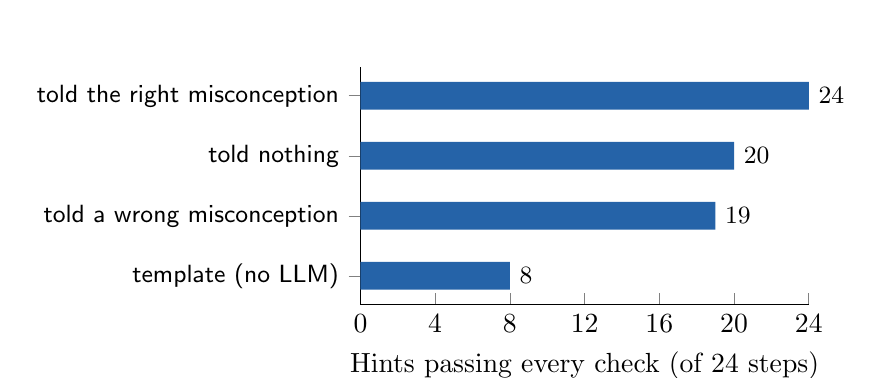
\begin{tikzpicture}
\begin{axis}[
  xbar, bar width=10pt,
  width=0.6\linewidth, height=4.6cm,
  xmin=0, xmax=24, xtick={0,4,8,12,16,20,24},
  xlabel={Hints passing every check (of 24 steps)},
  symbolic y coords={tpl,wrong,none,right},
  ytick={tpl,wrong,none,right}, y tick label style={font=\small\sffamily},
  yticklabels={template (no LLM), told a wrong misconception, told nothing, told the right misconception},
  enlarge y limits=0.16,
  axis x line*=bottom, axis y line*=left,
  nodes near coords, nodes near coords style={font=\small},
  every axis plot/.append style={draw=none},
]
\addplot[fill=withcritic] coordinates {(24,right) (20,none) (19,wrong) (8,tpl)};
\end{axis}
\end{tikzpicture}
\caption{The same hinter, given different diagnoses.}
\label{fig:hinter}
\end{figure}
\begin{table}[H]
\centering\small
\begin{tabular}{@{}lcccc@{}}
\toprule
Lines (author-labelled) & $n$ & Code only (hit / miss / abstain) & LLM only & As shipped \\
\midrule
standard & 13 & 13 / 0 / 0 & 10 / 2 / 1 & \best{13 / 0 / 0} \\
ambiguous (\code{a\^{}bc}, \code{1/2x}) & 11 & 0 / 0 / 11 & 10 / 1 / 0 & 10 / 1 / 0 \\
runs of letters & 8 & 1 / 0 / 7 & 8 / 0 / 0 & 8 / 0 / 0 \\
not maths & 8 & 8 / 0 / 0 & 6 / 2 / 0 & 6 / 2 / 0 \\
\midrule
all & 40 & 22 / 0 / 18 & 34 / 5 / 1 & \best{37 / 3 / 0} \\
\bottomrule
\end{tabular}
\caption{Reading the student's input.}
\label{tab:format}
\end{table}
On its own, the LLM rewrote two of the student's mistakes into correct maths: $3x + 4$ became $3(x + 4)$, and $3x^2$ became $(3x)^2$. Code accepted both, because only brackets changed, so the diagnoser would see no mistake. Reading with code first avoids this, and calls the model for 26 of 40 lines instead of all 40.
\begin{table}[H]
\centering\small
\begin{tabular}{@{}lcccc@{}}
\toprule
Variant & Right (107) & Wrong & None & Right topic (124) \\
\midrule
Code only & 77 (72\%) & 1 & 29 & 111 (90\%) \\
Code only, probe answered as the true rule predicts & 88 (82\%) & 1 & 18 & -- \\
As shipped (LLM fallback, Eedi off) & 77 (72\%) & 1 & 29 & 120 (97\%) \\
LLM only (every 3rd step: 42) & -- & -- & -- & 33/42 (79\%) \\
\bottomrule
\end{tabular}
\caption{Diagnosis on steps our rules generated. On the same 42 steps, the shipped tutor named the right topic for 41.}
\end{table}

There were 17 ties between rules, and answering the probe settled 11 of them to the right rule. Decimals (1 of 7) and scientific notation (0 of 7) are weak, largely because of the test itself: solve-back cannot split a written form such as $4.5 \times 10^4$.
\begin{table}[H]
\centering\small
\begin{tabular}{@{}lccc@{}}
\toprule
Critic & Right verdict & Faulty rejected (30) & Good rejected (12) \\
\midrule
Code checks only & 18 (43\%) & 6 & 0 \\
LLM review only & 39 (93\%) & 27 & 0 \\
\rowcolor{rowgray}As shipped & \best{39 (93\%)} & 27 & 0 \\
\bottomrule
\end{tabular}
\caption{The critic on author-labelled hints.}
\end{table}

The shipped critic caught every leak, every wrong-maths hint, every off-target hint and every too-advanced hint. It caught only 3 of 6 hints that do the step for the student, such as ``First, 1/2 is 3/6 and 1/3 is 2/6. Now add those two fractions.'' Reviewed three times with the cache off, every hint got the same verdict each time.
\begin{table}[H]
\centering\small
\begin{tabularx}{\linewidth}{@{}lP{3.3cm}Y@{}}
\toprule
\# & Ablation & Result \\
\midrule
A1 & LLM off & Rules and probes alone: \grp{has\_rule} top-1 1.00, \grp{known\_as\_text} 0.00; no leaks \\
A2 & Diagnoser's LLM off (\cond{nollmdiag}) & Topic accuracy 97\% $\to$ 90\% per step. In sessions, the same as full on \grp{has\_rule}; fewer budget stops (6 against 11 of 27) \\
A3 & Eedi off & Right misconception on Eedi's wrong answers 33\% $\to$ 5\% (40 steps) \\
A4 & Probes off (B2) & Top-1 1.00 $\to$ 0.72 offline (64 students), 1.00 $\to$ 0.52 with the LLM (8); 82\% $\to$ 72\% per step \\
-- & No diagnosis in feedback (\cond{nodiag}) & Learning 0.88 $\to$ 0.00 (by construction); budget stops 11 $\to$ 19 of 27; hinter 24/24 $\to$ 20/24 \\
-- & B1 (no critic, no memory) & Top-1 0.14; learning 0.00; leaks in 11 of 27 sessions \\
A6 & Critic's LLM review off & Right verdicts 93\% $\to$ 43\% \\
A8 & Slip checks off & Slips found 6/8 $\to$ 0/8 \\
A9 & T7 groups off & No change on 96 steps \\
A10 & Rewrites 0 / 1 / 2 & 20/24, 24/24, 24/24 approved \\
A5, A7 & Memory off; retrieval off & Not run \\
\bottomrule
\end{tabularx}
\caption{Ablations.}
\end{table}
\paragraph{What a user experiences.}
\begin{itemize}
  \item \textbf{A step code can settle} takes 0.003\,s at the median, with no model call.
  \item \textbf{One fresh model call} takes 5--7\,s at the median and 11--15\,s at the 90th percentile, on the free tier, from India.
  \item \textbf{A full analysis} takes about 12\,s for a mistake a rule explains (hinter and critic), and about 18\,s when the fallback runs.
  \item \textbf{Cost at paid prices:} about \$0.0005 per analysis with a rule, about \$0.001 with the fallback.
  \item \textbf{Invalid replies:} 2 of 749 calls were cut off (\code{MAX\_TOKENS}); both cases are now handled.
\end{itemize}

\section{Failures and design choices}
\begin{table}[H]
\centering\small
\begin{tabularx}{\linewidth}{@{}rP{4.4cm}YP{2.1cm}@{}}
\toprule
\# & Case & What happened & Stage \\
\midrule
1 & Typed \code{3x\^{}2} for $(3x)^2$ & LLM-only reading made it $(3x)^2$, hiding the mistake & input (LLM) \\
2 & Typed \code{hello} & Read as a named quantity; only the page's extra check catches it & input (LLM) \\
3 & \code{e\^{}2/a}, meaning $e^2 \div a$ & Read as $e^{2/a}$ & input (LLM) \\
4 & Eedi percentage step labelled 329 & The right rule fired, but the bank does not map it to 329 & bank mapping \\
5 & Eedi step $16 \to 16\%$ & A scientific-notation rule fired on a percentage & rules \\
6 & $6 \div 2 \times 3$ & Named the near-twin ``strictly sequential'' & rules \\
7 & ``1/2 is 3/6 and 1/3 is 2/6. Now add those.'' & Approved, although it does the step & critic \\
8 & $3(x+2) + 2(x+5) \to 3x+6+2x+5$ & Not called a slip & slips \\
9 & Students only Eedi describes & All 10 ran out of the token budget & budget \\
10 & B0, ``interpersonal influence'' student & Gave the answer at turn 2 & baseline \\
11 & $23 + 45 \to 14$, hinter told nothing & Hint about adding fractions & hinter \\
\bottomrule
\end{tabularx}
\caption{Failures, with the stage that broke.}
\label{tab:failures}
\end{table}
\begin{table}[H]
\centering\small
\begin{tabularx}{\linewidth}{@{}rP{4.3cm}YP{3.4cm}@{}}
\toprule
\# & Decision & Evidence & Strength \\
\midrule
1 & Code first, at most one LLM call per diagnosis & LLM-only reading rewrites mistakes; LLM-only diagnosis makes 19 wrong claims against 10 & \textbf{strong} \\
2 & Probes for tied rules & Top-1 1.00 against 0.72; 72\% $\to$ 82\% per step & moderate (simulated answers follow the rule exactly) \\
3 & Eedi pick only from a verified reading (T6) & Dropped picks 2/12 right, kept 11/20 & weak \\
4 & Near-duplicate groups (T7) & No effect on 96 steps & none yet \\
5 & Slips found by code & 6/8 slips, no false slips & moderate (hand cases) \\
6 & The critic as a gate & 0/27 leaks with it; 11/27 and 13/27 without; 93\% right verdicts & \textbf{strong} for leaks (by code) \\
7 & Hints aimed at the diagnosis, with certainty levels & Right 24/24, none 20/24, wrong 19/24 & moderate \\
8 & Hybrid textbook search & Right section in the top 3: 97\% against 87\% for one method (earlier study) & moderate (not re-run) \\
9 & 20 in-topic Eedi names & The right name is offered for 85\% of steps & moderate \\
10 & Shortlister v2 & 5\% $\to$ 33\% with Eedi on held-out data & \textbf{strong} \\
11 & Gemini for the final runs & Better than Qwen 7B on vLLM (earlier study) & moderate \\
12 & 20,000-token session budget & Hit by every text-only student & \textbf{evidence against} \\
13 & One rewrite on the page, two in the runner & 24/24 approved by the second attempt & moderate \\
\bottomrule
\end{tabularx}
\caption{Each decision, its evidence and how strong that evidence is.}
\label{tab:choices}
\end{table}
\section{Reproducing the results}

Every run used commit \code{1f65ae2}.
\begin{itemize}
  \item Scripts: \code{eval/report\_eval.py} and \code{eval/report\_tables.py}.
  \item Logs: \code{runs/report/}, outside version control.
\end{itemize}
Calls are at temperature 0 with a cache, so a rerun reproduces the same outputs without new requests.

\begin{small}
\begin{verbatim}
PYTHONPATH=. python eval/report_eval.py format
PYTHONPATH=. python eval/report_eval.py diagnosis
PYTHONPATH=. python eval/report_eval.py diagnosis --eedi   # GPU
PYTHONPATH=. python eval/report_eval.py slips
PYTHONPATH=. python eval/report_eval.py critic
PYTHONPATH=. python eval/report_eval.py hinter
PYTHONPATH=. python eval/report_eval.py sessions --offline \
    --sample all --sessions 2 --conditions full,b2,nodiag
PYTHONPATH=. python eval/report_eval.py sessions \
    --conditions full,b0,nodiag,b1,b2,nollmdiag
PYTHONPATH=. python eval/report_tables.py > runs/report/tables.md
\end{verbatim}
\end{small}

\end{document}
